\documentclass[11pt]{report}
\usepackage[utf8]{inputenc}
 \usepackage{listings}
 \usepackage{color}
 \usepackage{fancyhdr}
 \usepackage{graphicx}
\pagestyle{fancy}

 \lhead{Geoffrey PERRIN \\ Océane DUBOIS}
 \rhead{MI01 - TP02 : VHDL séquentiel}
 \rfoot{}



\definecolor{dkgreen}{rgb}{0,0.6,0}
\definecolor{gray}{rgb}{0.5,0.5,0.5}
\definecolor{mauve}{rgb}{0.58,0,0.82}

\lstset{frame=tb,
  language=vhdl,
  aboveskip=3mm,
  belowskip=3mm,
  showstringspaces=false,
  columns=flexible,
  basicstyle={\small\ttfamily},
  numbers=none,
  numberstyle=\tiny\color{gray},
  keywordstyle=\color{blue},
  commentstyle=\color{dkgreen},
  stringstyle=\color{mauve},
  breaklines=true,
  breakatwhitespace=true,
  tabsize=3
}

 
%Gummi|065|=)
\title{\textbf{TP02 - VHDL séquentiel}
\author{Geoffrey PERRIN \\ Océane DUBOIS\\}
\date{}}

\begin{document}

\maketitle

\newpage


\section{Compteur de 2 bits}

Dans cet exercice on cherche à implémenter le  modèle VHDL d'un compteur synchrone à 2 bits, 
On utilisera : \begin{itemize}
	 \item  une entrée  pour le reset : PB\_1. Cette entrée est un bouton qui remet le compteur à 0 si on le met à '1'.
	\item un signal d'entrée (un bouton) PB\_0 pôur l'horloge qui incrémente le compteur lorsqu'on le met à 1.
	 \item le signal LED\_10 comme signal de sortie, qui est un groupe de 2 led qui permet d'afficher le resultat du compteur.
	 
	\end{itemize}

\medskip

Chaque fois que l'on appuie sur le bouton, le compteur est incrémenté de 1. Le résultat est affiché grâce aux LED. Si la valeur du compteur dépasse 3, le compteur est remis à 0 car la carte affiche le résultat du compteur modulo 2. Sinon le bouton reset (PB\_1), permet de remettre le compteur à 0.

\medskip

On pensera à se synchroniser sur le front montant de l'horloge.

\subsection{ a) Ecriture du programme en VHDL}

Voici le programme de l'exercice 1. On a supprimé les premières instructions dans un soucis de clareté du programme.

Voici d'abord le code du reset synchrone. On a ici un reset synchrone car le signal du reset n'est pas dans la liste de sensibilité du process et qu'il ne prend effet que si le signal PB\_0 change d'état et passe à 1.

\begin{lstlisting}
entity compteur is
PORT(PB_0,PB_1:IN BIT;
		LED_10: OUT INTEGER RANGE 0 to 3);
end compteur;

architecture Behavioral of compteur is

begin
PROCESS(PB_0)
VARIABLE resultat:INTEGER range 0 to 3;
BEGIN
	IF(PB_0'EVENT and PB_0='1') THEN
		IF PB_1 = '0' THEN 
			resultat := resultat + 1;
		ELSE
			resultat := 0;
		END IF;
	END IF;

LED_10 <= resultat;

END PROCESS;

end Behavioral;

\end{lstlisting}

Et voici maintenant le code du reset asynchrone. On a simplement passé le signal du reset dans la liste de sensibilité du process et on peut activer le reset indépendemment du signal PB\_0, puisque l'activation du reset ne se trouve plus à l'intérieur de la condition "IF(PB\_0'EVENT and PB\_0='1') THEN". Il peut donc se déclancher indépendamment de l'activation du compteur. 


\begin{lstlisting}
entity compteur is
PORT(PB_0,PB_1:IN BIT;
		LED_10: OUT INTEGER RANGE 0 to 3);
end compteur;

architecture Behavioral of compteur is

begin
PROCESS(PB_0, PB_1)
VARIABLE resultat:INTEGER range 0 to 3;
BEGIN
IF (PB_1 = '1') THEN
	resultat := 0;
ELSE IF(PB_0'EVENT and PB_0='1') THEN

			resultat := resultat + 1;
end if;
END IF;

LED_10 <= resultat;

END PROCESS;

END Behavioral;

\end{lstlisting}

Une fois que les deux programmes sont écrits on procède à la synthèse des programmes. 
 
 \subsection{ b) Synthèse du code VHDL }
 
 Avertissement sur PB\_0 ???????
 
 Voic la synthèse avec le code du reset synchrone :
 \begin{figure}[h]
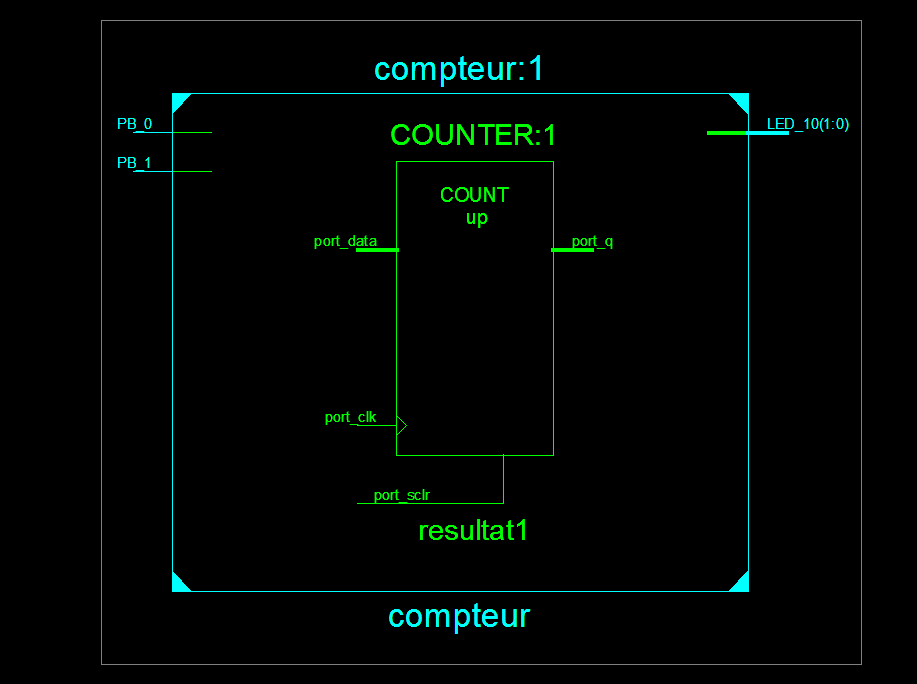
\includegraphics[width=8cm]{TP02-3.PNG}
\caption{Schéma RTL du compteur avec reset synchrone}
\end{figure}

On remarque bien les deux entrée PB\_0 et PB\_1, le compteur au milieu du composant et la LED\_10 qui correspond à la sortie. 

Voici maintenant la vue technologique du code avec le reset synchrone : 

\begin{figure}[h]
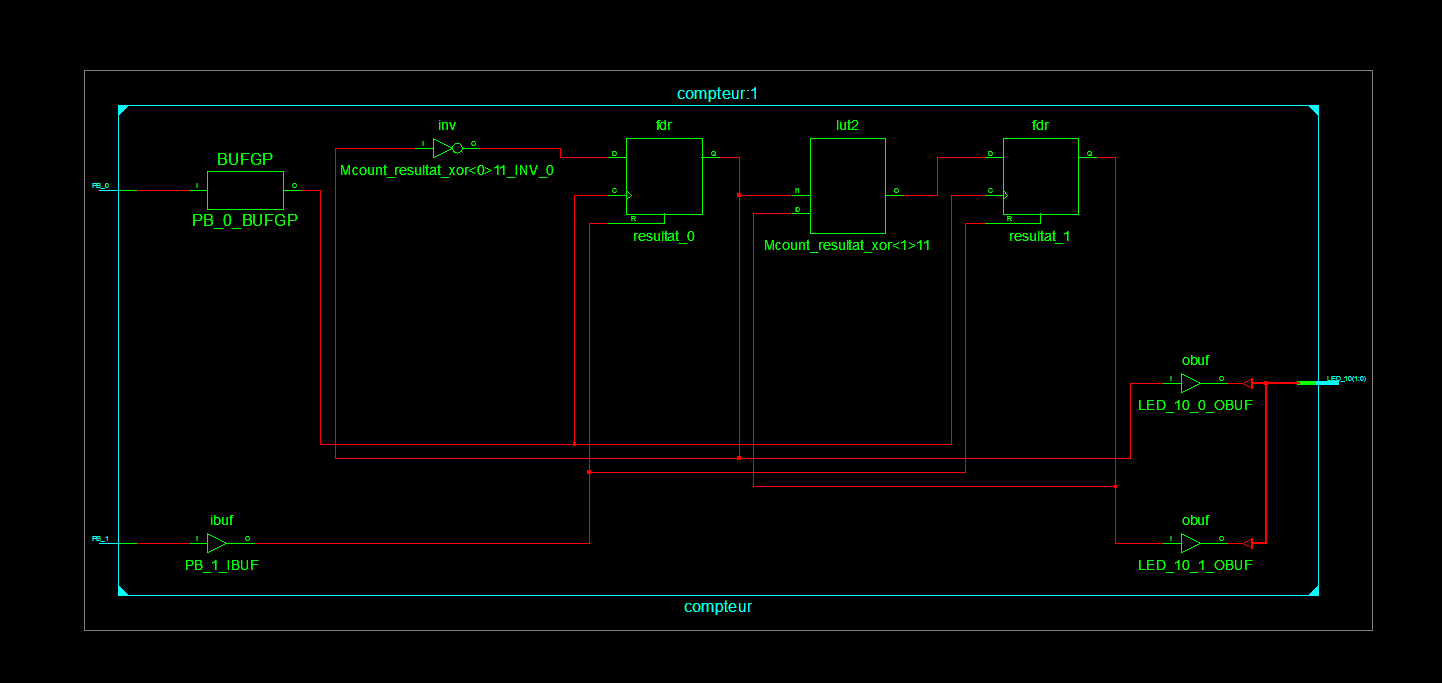
\includegraphics[width=8cm]{TP02-4.PNG}
\caption{Schéma technologique du compteur avec reset synchrone}
\end{figure}

COMMENTAIRE ????????? 
 
\subsection{ c) Simulation du circuit}

Ensuite nous effectuons la simulation du circuit grâce au logiciel. 
En faisant varier les 2 signaux d'entrée voici le résultat que nous obtenons.

\begin{figure}[h]
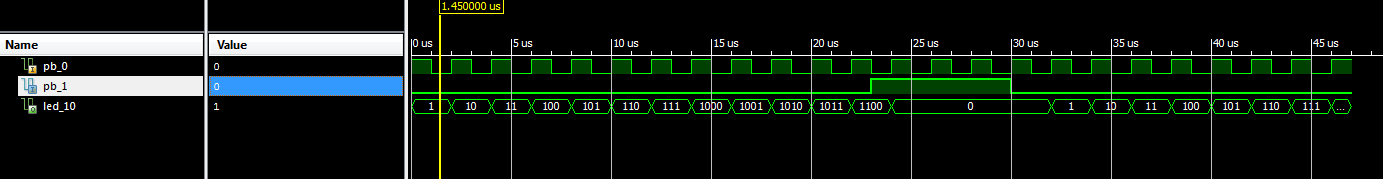
\includegraphics[width=15cm]{TP02-1.PNG}
\caption{Simulation du compteur avec reset synchrone}
\end{figure}

Lors de la simulation avec l'horloge synchrone on remarque que lorsque le reset est activé, on doit attendre que le signal d'entrée PB\_0 soit passé à '1' pour que le compteur repasse à 0, tant que le signal d'entre PB\_0 n'est pas passé à 1, le reset ne prend pas effet.

Ce n'est pas le cas avec un reset asynchrone, dont voici la simulation :

\begin{figure}[h]
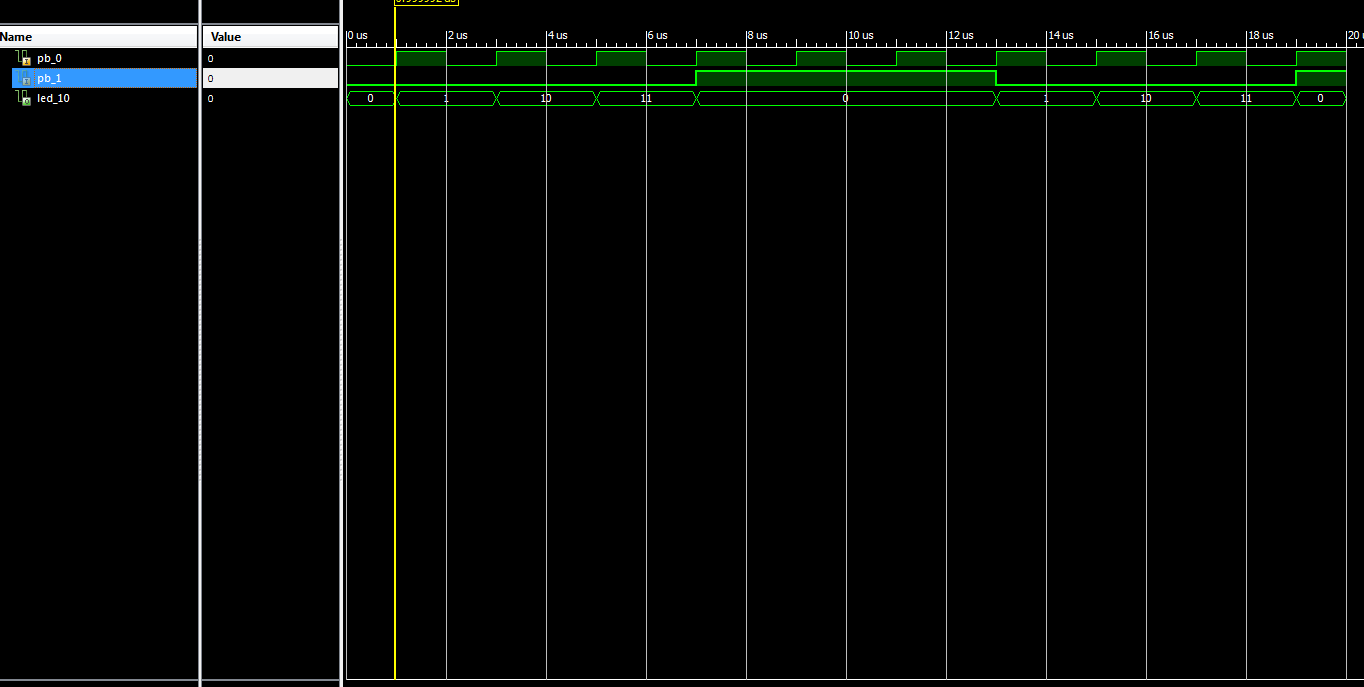
\includegraphics[width=15cm]{TP02-5.PNG}
\caption{Simulation du compteur avec reset asynchrone}
\end{figure}

Ici on peut voir que le reset prend effet dès sont activation, on n'a pas besoin que PB\_0 soit activé. 

  
   \subsection{ d) programmation du FPGA}
   
   
 

\section{Détecteur de code}

Dans cet exercice on réalisera un détécteur pour le code 11010. Si le code est détecté, une alarme est activée. On utilisera les signaux :
\begin{itemize}
	\item BP\_0 pour l'horloge
	\item SW\_0 pour la ligne de transmission
	\item LED\_0 pour symboliser l'alarme
	\item LED\_7654 pour afficher l'état

\end{itemize}

Dans cette première modélisation on supposera qu'une fausse entrée implique de tout recommencer. 

\subsection{Ecriture du code VHDL}

\begin{lstlisting}
entity exercice2 is
	PORT(BP_0, SW_0 : IN BIT;
		LED_0 : OUT BIT);
end exercice2;

architecture detecteur of exercice2 is
begin
process(BP_0)
variable state : INTEGER RANGE 0 to 5;
begin
	if(PB_0'Event and PB_0 = '1') then
		case state is
			when 0 => if (SW_0 = '1') then 
						state := 1; 
						LED_0 <= '0'; 
					  end if;
			when 1 => if (SW_0 = '1') then 
						state := 2; 
					  else LED_0 <= '1'; 
						state :=0; 
					  end if;
			when 2 => if (SW_0 = '0') then 
						state := 3; 
					  else 
					  	LED_0 <= '1';
					  	 state :=0; 
					  end if;
			when 3 => if (SW_0 = '1') then 
						state := 4; 
					  else
					  	 LED_0 <= '1'; 
					  	 state :=0; 
					  end if;
			when 4 => if (SW_0 = '0') then 
						state := 5; 
					else LED_0 <= '1'; 
						state :=0;
					end if;
			when others => state := 0;
		end case;
	LED_7654 <= state;
	end if;

end process;

end detecteur;

\end{lstlisting}


\subsection{ b) Synthèse du code VHDL }
 
  \subsection{ c) Simulation du circuit}
  
  Nombre de bits utilisés par le detecteur et sous quelle forme
  Equation de génération de la sortie
  
  
   \subsection{ d) programmation du FPGA}


\section{Détecteur de code avec une fausse entrée négligée}

Dans cet exercice on réalisera un détécteur pour le code 11010. Si le code est détecté, une alarme est activée. On utilisera les signaux :
\begin{itemize}
	\item BP\_0 pour l'horloge
	\item SW\_0 pour la ligne de transmission
	\item LED\_0 pour symboliser l'alarme
	\item LED\_7654 pour afficher l'état

\end{itemize}

Dans cette première modélisation on supposera qu'une fausse entrée est négligée. 

\subsection{Ecriture du code VHDL}

\begin{lstlisting}
entity exercice3 is
	PORT(BP_0, SW_0 : IN BIT;
		LED_0 : OUT BIT);
end exercice3;

architecture detecteur of exercice3 is
begin
process(BP_0)
variable state : INTEGER RANGE 0 to 5;
begin
	if(PB_0'Event and PB_0 = '1') then
		case state is
			when 0 => if (SW_0 = '1') then 
						state := 1; 
						LED_0 <= '0'; 
					  end if;
			when 1 => if (SW_0 = '1') then 
						state := 2; 
					  else 
					  	LED_0 <= '1'; 
						state :=1; 
					  end if;
			when 2 => if (SW_0 = '0') then 
						state := 3; 
					  else 
					  	LED_0 <= '1';
					  	 state :=2; 
					  end if;
			when 3 => if (SW_0 = '1') then 
						state := 3; 
					  else
					  	 LED_0 <= '1'; 
					  	 state :=3; 
					  end if;
			when 4 => if (SW_0 = '0') then 
						state := 5; 
					else LED_0 <= '1'; 
						state :=4;
					end if;
			when others => state := 0;
		end case;
	LED_7654 <= state;
	end if;

end process;

end detecteur;

\end{lstlisting}


\subsection{ b) Synthèse du code VHDL }
 
  \subsection{ c) Simulation du circuit}
  
  Nombre de bits utilisés par le detecteur et sous quelle forme
  Equation de génération de la sortie
  
  
   \subsection{ d) programmation du FPGA}


\end{document}





























